% Created by tikzDevice version 0.12.3.1 on 2022-03-06 11:17:41
% !TEX encoding = UTF-8 Unicode
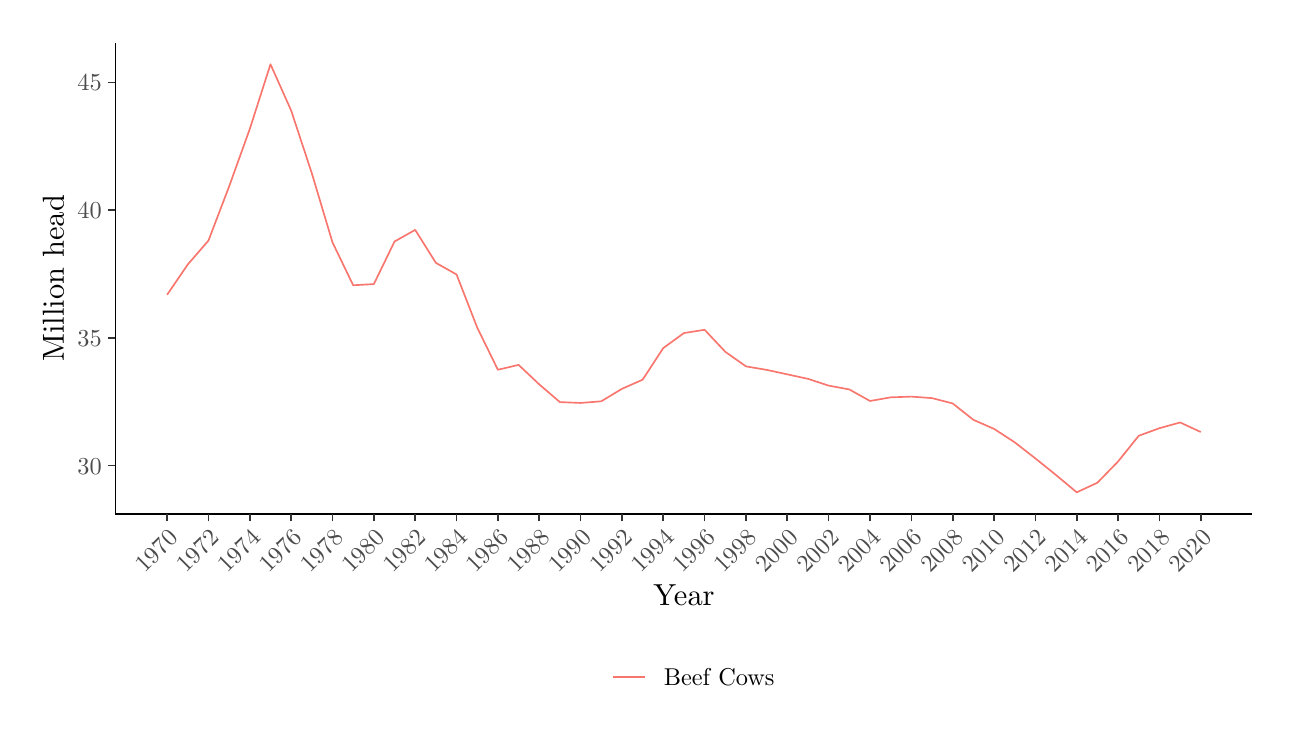
\begin{tikzpicture}[x=1pt,y=1pt]
\definecolor{fillColor}{RGB}{255,255,255}
\path[use as bounding box,fill=fillColor,fill opacity=0.00] (0,0) rectangle (448.07,252.94);
\begin{scope}
\path[clip] (  0.00,  0.00) rectangle (448.07,252.94);
\definecolor{drawColor}{RGB}{255,255,255}
\definecolor{fillColor}{RGB}{255,255,255}

\path[draw=drawColor,line width= 0.6pt,line join=round,line cap=round,fill=fillColor] (  0.00,  0.00) rectangle (448.07,252.94);
\end{scope}
\begin{scope}
\path[clip] ( 31.71, 77.31) rectangle (442.57,247.44);
\definecolor{fillColor}{RGB}{255,255,255}

\path[fill=fillColor] ( 31.71, 77.31) rectangle (442.57,247.44);
\definecolor{drawColor}{RGB}{248,118,109}

\path[draw=drawColor,line width= 0.6pt,line join=round] ( 50.39,156.43) --
	( 57.86,167.39) --
	( 65.33,176.00) --
	( 72.80,195.58) --
	( 80.27,216.36) --
	( 87.74,239.71) --
	( 95.21,222.99) --
	(102.68,200.31) --
	(110.15,175.34) --
	(117.62,159.86) --
	(125.09,160.28) --
	(132.56,175.66) --
	(140.03,179.87) --
	(147.50,167.96) --
	(154.97,163.76) --
	(162.44,144.57) --
	(169.91,129.32) --
	(177.38,131.09) --
	(184.85,124.05) --
	(192.32,117.64) --
	(199.79,117.33) --
	(207.26,117.93) --
	(214.73,122.43) --
	(222.20,125.73) --
	(229.67,137.16) --
	(237.14,142.59) --
	(244.61,143.77) --
	(252.08,135.82) --
	(259.55,130.54) --
	(267.02,129.29) --
	(274.49,127.67) --
	(281.96,126.04) --
	(289.43,123.60) --
	(296.90,122.21) --
	(304.38,118.04) --
	(311.85,119.36) --
	(319.32,119.62) --
	(326.79,119.08) --
	(334.26,117.15) --
	(341.73,111.23) --
	(349.20,107.96) --
	(356.67,103.10) --
	(364.14, 97.28) --
	(371.61, 91.27) --
	(379.08, 85.04) --
	(386.55, 88.51) --
	(394.02, 96.19) --
	(401.49,105.48) --
	(408.96,108.21) --
	(416.43,110.28) --
	(423.90,106.83);
\end{scope}
\begin{scope}
\path[clip] (  0.00,  0.00) rectangle (448.07,252.94);
\definecolor{drawColor}{RGB}{0,0,0}

\path[draw=drawColor,line width= 0.6pt,line join=round] ( 31.71, 77.31) --
	( 31.71,247.44);
\end{scope}
\begin{scope}
\path[clip] (  0.00,  0.00) rectangle (448.07,252.94);
\definecolor{drawColor}{gray}{0.30}

\node[text=drawColor,anchor=base east,inner sep=0pt, outer sep=0pt, scale=  0.88] at ( 26.76, 91.64) {30};

\node[text=drawColor,anchor=base east,inner sep=0pt, outer sep=0pt, scale=  0.88] at ( 26.76,137.80) {35};

\node[text=drawColor,anchor=base east,inner sep=0pt, outer sep=0pt, scale=  0.88] at ( 26.76,183.95) {40};

\node[text=drawColor,anchor=base east,inner sep=0pt, outer sep=0pt, scale=  0.88] at ( 26.76,230.11) {45};
\end{scope}
\begin{scope}
\path[clip] (  0.00,  0.00) rectangle (448.07,252.94);
\definecolor{drawColor}{gray}{0.20}

\path[draw=drawColor,line width= 0.6pt,line join=round] ( 28.96, 94.67) --
	( 31.71, 94.67);

\path[draw=drawColor,line width= 0.6pt,line join=round] ( 28.96,140.83) --
	( 31.71,140.83);

\path[draw=drawColor,line width= 0.6pt,line join=round] ( 28.96,186.98) --
	( 31.71,186.98);

\path[draw=drawColor,line width= 0.6pt,line join=round] ( 28.96,233.14) --
	( 31.71,233.14);
\end{scope}
\begin{scope}
\path[clip] (  0.00,  0.00) rectangle (448.07,252.94);
\definecolor{drawColor}{RGB}{0,0,0}

\path[draw=drawColor,line width= 0.6pt,line join=round] ( 31.71, 77.31) --
	(442.57, 77.31);
\end{scope}
\begin{scope}
\path[clip] (  0.00,  0.00) rectangle (448.07,252.94);
\definecolor{drawColor}{gray}{0.20}

\path[draw=drawColor,line width= 0.6pt,line join=round] ( 50.39, 74.56) --
	( 50.39, 77.31);

\path[draw=drawColor,line width= 0.6pt,line join=round] ( 65.33, 74.56) --
	( 65.33, 77.31);

\path[draw=drawColor,line width= 0.6pt,line join=round] ( 80.27, 74.56) --
	( 80.27, 77.31);

\path[draw=drawColor,line width= 0.6pt,line join=round] ( 95.21, 74.56) --
	( 95.21, 77.31);

\path[draw=drawColor,line width= 0.6pt,line join=round] (110.15, 74.56) --
	(110.15, 77.31);

\path[draw=drawColor,line width= 0.6pt,line join=round] (125.09, 74.56) --
	(125.09, 77.31);

\path[draw=drawColor,line width= 0.6pt,line join=round] (140.03, 74.56) --
	(140.03, 77.31);

\path[draw=drawColor,line width= 0.6pt,line join=round] (154.97, 74.56) --
	(154.97, 77.31);

\path[draw=drawColor,line width= 0.6pt,line join=round] (169.91, 74.56) --
	(169.91, 77.31);

\path[draw=drawColor,line width= 0.6pt,line join=round] (184.85, 74.56) --
	(184.85, 77.31);

\path[draw=drawColor,line width= 0.6pt,line join=round] (199.79, 74.56) --
	(199.79, 77.31);

\path[draw=drawColor,line width= 0.6pt,line join=round] (214.73, 74.56) --
	(214.73, 77.31);

\path[draw=drawColor,line width= 0.6pt,line join=round] (229.67, 74.56) --
	(229.67, 77.31);

\path[draw=drawColor,line width= 0.6pt,line join=round] (244.61, 74.56) --
	(244.61, 77.31);

\path[draw=drawColor,line width= 0.6pt,line join=round] (259.55, 74.56) --
	(259.55, 77.31);

\path[draw=drawColor,line width= 0.6pt,line join=round] (274.49, 74.56) --
	(274.49, 77.31);

\path[draw=drawColor,line width= 0.6pt,line join=round] (289.43, 74.56) --
	(289.43, 77.31);

\path[draw=drawColor,line width= 0.6pt,line join=round] (304.38, 74.56) --
	(304.38, 77.31);

\path[draw=drawColor,line width= 0.6pt,line join=round] (319.32, 74.56) --
	(319.32, 77.31);

\path[draw=drawColor,line width= 0.6pt,line join=round] (334.26, 74.56) --
	(334.26, 77.31);

\path[draw=drawColor,line width= 0.6pt,line join=round] (349.20, 74.56) --
	(349.20, 77.31);

\path[draw=drawColor,line width= 0.6pt,line join=round] (364.14, 74.56) --
	(364.14, 77.31);

\path[draw=drawColor,line width= 0.6pt,line join=round] (379.08, 74.56) --
	(379.08, 77.31);

\path[draw=drawColor,line width= 0.6pt,line join=round] (394.02, 74.56) --
	(394.02, 77.31);

\path[draw=drawColor,line width= 0.6pt,line join=round] (408.96, 74.56) --
	(408.96, 77.31);

\path[draw=drawColor,line width= 0.6pt,line join=round] (423.90, 74.56) --
	(423.90, 77.31);
\end{scope}
\begin{scope}
\path[clip] (  0.00,  0.00) rectangle (448.07,252.94);
\definecolor{drawColor}{gray}{0.30}

\node[text=drawColor,rotate= 45.00,anchor=base east,inner sep=0pt, outer sep=0pt, scale=  0.88] at ( 54.67, 68.07) {1970};

\node[text=drawColor,rotate= 45.00,anchor=base east,inner sep=0pt, outer sep=0pt, scale=  0.88] at ( 69.61, 68.07) {1972};

\node[text=drawColor,rotate= 45.00,anchor=base east,inner sep=0pt, outer sep=0pt, scale=  0.88] at ( 84.55, 68.07) {1974};

\node[text=drawColor,rotate= 45.00,anchor=base east,inner sep=0pt, outer sep=0pt, scale=  0.88] at ( 99.49, 68.07) {1976};

\node[text=drawColor,rotate= 45.00,anchor=base east,inner sep=0pt, outer sep=0pt, scale=  0.88] at (114.44, 68.07) {1978};

\node[text=drawColor,rotate= 45.00,anchor=base east,inner sep=0pt, outer sep=0pt, scale=  0.88] at (129.38, 68.07) {1980};

\node[text=drawColor,rotate= 45.00,anchor=base east,inner sep=0pt, outer sep=0pt, scale=  0.88] at (144.32, 68.07) {1982};

\node[text=drawColor,rotate= 45.00,anchor=base east,inner sep=0pt, outer sep=0pt, scale=  0.88] at (159.26, 68.07) {1984};

\node[text=drawColor,rotate= 45.00,anchor=base east,inner sep=0pt, outer sep=0pt, scale=  0.88] at (174.20, 68.07) {1986};

\node[text=drawColor,rotate= 45.00,anchor=base east,inner sep=0pt, outer sep=0pt, scale=  0.88] at (189.14, 68.07) {1988};

\node[text=drawColor,rotate= 45.00,anchor=base east,inner sep=0pt, outer sep=0pt, scale=  0.88] at (204.08, 68.07) {1990};

\node[text=drawColor,rotate= 45.00,anchor=base east,inner sep=0pt, outer sep=0pt, scale=  0.88] at (219.02, 68.07) {1992};

\node[text=drawColor,rotate= 45.00,anchor=base east,inner sep=0pt, outer sep=0pt, scale=  0.88] at (233.96, 68.07) {1994};

\node[text=drawColor,rotate= 45.00,anchor=base east,inner sep=0pt, outer sep=0pt, scale=  0.88] at (248.90, 68.07) {1996};

\node[text=drawColor,rotate= 45.00,anchor=base east,inner sep=0pt, outer sep=0pt, scale=  0.88] at (263.84, 68.07) {1998};

\node[text=drawColor,rotate= 45.00,anchor=base east,inner sep=0pt, outer sep=0pt, scale=  0.88] at (278.78, 68.07) {2000};

\node[text=drawColor,rotate= 45.00,anchor=base east,inner sep=0pt, outer sep=0pt, scale=  0.88] at (293.72, 68.07) {2002};

\node[text=drawColor,rotate= 45.00,anchor=base east,inner sep=0pt, outer sep=0pt, scale=  0.88] at (308.66, 68.07) {2004};

\node[text=drawColor,rotate= 45.00,anchor=base east,inner sep=0pt, outer sep=0pt, scale=  0.88] at (323.60, 68.07) {2006};

\node[text=drawColor,rotate= 45.00,anchor=base east,inner sep=0pt, outer sep=0pt, scale=  0.88] at (338.54, 68.07) {2008};

\node[text=drawColor,rotate= 45.00,anchor=base east,inner sep=0pt, outer sep=0pt, scale=  0.88] at (353.48, 68.07) {2010};

\node[text=drawColor,rotate= 45.00,anchor=base east,inner sep=0pt, outer sep=0pt, scale=  0.88] at (368.42, 68.07) {2012};

\node[text=drawColor,rotate= 45.00,anchor=base east,inner sep=0pt, outer sep=0pt, scale=  0.88] at (383.36, 68.07) {2014};

\node[text=drawColor,rotate= 45.00,anchor=base east,inner sep=0pt, outer sep=0pt, scale=  0.88] at (398.30, 68.07) {2016};

\node[text=drawColor,rotate= 45.00,anchor=base east,inner sep=0pt, outer sep=0pt, scale=  0.88] at (413.24, 68.07) {2018};

\node[text=drawColor,rotate= 45.00,anchor=base east,inner sep=0pt, outer sep=0pt, scale=  0.88] at (428.18, 68.07) {2020};
\end{scope}
\begin{scope}
\path[clip] (  0.00,  0.00) rectangle (448.07,252.94);
\definecolor{drawColor}{RGB}{0,0,0}

\node[text=drawColor,anchor=base,inner sep=0pt, outer sep=0pt, scale=  1.10] at (237.14, 44.09) {Year};
\end{scope}
\begin{scope}
\path[clip] (  0.00,  0.00) rectangle (448.07,252.94);
\definecolor{drawColor}{RGB}{0,0,0}

\node[text=drawColor,rotate= 90.00,anchor=base,inner sep=0pt, outer sep=0pt, scale=  1.10] at ( 13.08,162.38) {Million head};
\end{scope}
\begin{scope}
\path[clip] (  0.00,  0.00) rectangle (448.07,252.94);
\definecolor{fillColor}{RGB}{255,255,255}

\path[fill=fillColor] (198.91,  5.50) rectangle (275.37, 30.95);
\end{scope}
\begin{scope}
\path[clip] (  0.00,  0.00) rectangle (448.07,252.94);
\definecolor{drawColor}{RGB}{248,118,109}

\path[draw=drawColor,line width= 0.6pt,line join=round] (211.36, 18.23) -- (222.92, 18.23);
\end{scope}
\begin{scope}
\path[clip] (  0.00,  0.00) rectangle (448.07,252.94);
\definecolor{drawColor}{RGB}{0,0,0}

\node[text=drawColor,anchor=base west,inner sep=0pt, outer sep=0pt, scale=  0.88] at (229.87, 15.20) {Beef Cows};
\end{scope}
\end{tikzpicture}
